\section{Algorithm}

% Notation for frequently used matrices and indices. Defined in spdistnmfsc17.tex, commented out here for reference.
% \newcommand{\mat}[1]{\mathbf{#1}}  % Denote a matrix
% \newcommand{\matt}[1]{\mathbf{\tilde{#1}}}  % Denote a matrix with hat
% \newcommand{\Am}{\mat{A}} % Input sparse matrix
% \newcommand{\Amp}{\mat{A}_p} % Input sparse matrix
% \newcommand{\Wm}{\mat{W}} % Factor matrix
% \newcommand{\Wmt}{\matt{W}} % AH result
% \newcommand{\Hm}{\mat{H}} % Factor matrix
% \newcommand{\Hmt}{\matt{H}} % WtA result
% \newcommand{\Ip}{\mathcal{I}_p}
% \newcommand{\Jp}{\mathcal{J}_p}
% \newcommand{\Fp}{\mathcal{F}_p}
% \newcommand{\Gp}{\mathcal{G}_p}

Here, we first introduce our parallel NMF algorithm that operates on a partition of the matrices $\Am$, $\Wm$, and $\Hm$.
For a given partition, we describe how parallel computations and communications take place within the algorithm, and illustrate computational and communication costs associated with a partition.
In doing so, we elaborate the advantages of our parallelization scheme compared with the state of the art.
We then discuss efficient partitioning strategies to better establish computational load balance and reduce communication.

\subsection{Distributed Parallel Sparse NMF Algorithm}

\begin{algorithm}
\caption{\distspnmf: \distspnmffull}
\label{alg:distnmf}
  \begin{algorithmic}[1]
    \setcounter{ALC@unique}{0}
    \REQUIRE {$\Amp$: An $m \times n$ sparse matrix \\
      $\Ip$,$\Jp$: Set of rows/columns of $\Wm$ and $\Hm$ owned by process $p$ \\
      $\Fp$,$\Gp$: Footprints of process $p$ on $\Wm$ and $\Hm$ \\
      $\Wm(\Ip,:)$,$\Hm(:,\Jp)$: Owned rows and columns of initial $\Wm$ and $\Hm$ \\
      $k$: The NMF rank}
    \ENSURE {Process $p$ gets the final value of $\Wm(\Ip,:)$ and $\Hm(:,\Jp)$}
      \REPEAT
        \STATE $\Cexpand (\Hm(:,\Gp))$ \label{line:exph}
        \STATE $\Wmt(\Fp, :) \gets \Amp \Hm(:, \Gp)$ \label{line:ah}
        \STATE $\Cfold(\Wmt(\Fp, :))$ \label{line:foldw}
        \STATE $\Hmgr \gets \textsc{All-Reduce}(\Hm(:, \Jp) \Hm(:, \Jp)^T)$ \label{line:hmgr}
        \STATE $\Wm(\Ip, :) \gets \textsc{Nnls}(\Hmgr, \Wmt(\Ip, :))$ \label{line:wmnnls}
        \STATE $\Cexpand(\Wm(\Fp, :))$ \label{line:expw}
        \STATE $\Hmt(:, \Gp) \gets \Wm(\Fp, :)^T \Amp$ \label{line:wta}
        \STATE $\Cfold(\Hmt(:, \Gp))$ \label{line:foldh}
        \STATE $\Wmgr \gets \textsc{All-Reduce}(\Wm(\Ip, :)^T \Wm(\Ip, :))$ \label{line:wmgr}
        \STATE $\Hm(\Jp, :) \gets \textsc{Nnls}(\Wmgr, \Hmt(\Jp, :))$ \label{line:hmnnls}
      \UNTIL{convergence or maximum number of iterations}
  \end{algorithmic}
\end{algorithm}

Parallellizing NMF involves partitioning data and computational tasks to processes, and communicating results wherever necessary, just as any parallel algorithm.
Specifically for NMF, one needs to partition the sparse matrix $\Am$ as well as the factor matrices $\Wm$ and $\Hm$, where the former partitioning distributes the computational load of sparse matrix-dense matrix multiplications $\Am \Hm$ and $\Wm^T \Am$, whereas the latter divides the workload of NNLS computations to processes.
We provide the execution of our parallel algorithm for computing a rank-$k$ NMF of a sparse matrix $\Am \in \R^{m \times n}$ in \cref{alg:distnmf}, which is executed by each process $p$ for $1 \le p \le P$.
The algorithm starts with an arbitrary partition of the input matrix and the factor matrices; process $p$ owns the submatrices $\Wm(\Ip, :)$ and $\Hm(:, \Jp)$ as well as the nonzero elements of the sparse matrix $\Am_p$ where $\Am = \bigcup_{i=1}^{P}\Am_i$, i.e., $\Am_1, \dots, \Am_p$ partitions the nonzeros of $\Am$.
The sets $\Fp$ and $\Gp$ denote the ``footprints'' of the process $p$ on the rows and the columns of matrices $\Wm$ and $\Hm$, respectively, in the course of the algorithm.
That is, we have $i \in \Fp$ or $j \in \Gp$ if only if $i \in \Ip$ or $j \in \Jp$~(row/column is owned), or there is a nonzero element $a_{i,j} \in \Amp$~(row/column is used in local computations).
At each iteration, the process $p$ is responsible for gathering the new value of submatrices $\Wm(\Ip, :)$ and $\Hm(:, \Jp)$, and sending these values to processes in need.

In an iteration of \cref{alg:distnmf}, each process $p$ possesses three types of computational tasks as well as associated pre- and post-communication steps.
The first task involves performing sparse matrix-dense matrix multiplications $\Am_p \Hm(:, \Gp)$ and $\Wm(\Fp, :)^T \Am_p$, whose results are stored in distributed matrices $\Wmt$ and $\Hmt$, which follow the same row-/column-wise data distribution as $\Wm$ and $\Hm$.
Note that carrying out these multiplications must be preceded by a communication step where each process $p$ gets the submatrices $\Hm(:, \Gp \setminus \Jp)$ and $\Wm(\Fp \setminus \Ip, :)$ that are accessed by entries of $\Amp$, and this step is performed at \cref{line:exph,line:expw}.
These multiplications performed by each process $p$ generate partial results for the set $\Fp$ and $\Gp$ of rows of $\Wmt$ and columns of $\Hmt$, respectively, which is highlighted at \cref{line:ah,line:wta}.
Indeed, partial results for the submatrices $\Wmt(\Fp \setminus \Ip, :)$ and $\Hmt(:, \Gp \setminus \Jp)$ correspond to rows and columns owned by other processes; hence, they need to be communicated.
The results for $\Wmt(\Ip, :)$ and $\Hmt(:, \Jp)$, however, should be kept locally, and all partial results for these matrix rows and columns generated by other processes should similarly be received and accumulated in order to obtain the final value for these owned portions.
The second task is to compute the Gram matrices $\Hmgr = \Hm \Hm^T$ and $\Wmgr = \Wm^T \Wm$ of size $k \times k$, and making these matrices available to all processes, which is performed at \cref{line:hmgr,line:wmgr}.
This is done in a row-parallel dense matrix multiplication step, in which the process $p$ computes $\Hm(:, \Jp) \Hm^T(:, \Jp)$ and $\Wm^T(\Ip, :) \Wm(\Ip, :)$, followed by an \textsc{All-Reduce} communication of these partial multiplications.
The third task pertains to updating the factor matrices $\Wm$ and $\Hm$ using matrices $\Wmt$ and $\Hmgr$, or $\Hmt$ and $\Wmgr$, which takes place at \cref{line:wmnnls,line:hmnnls}.
This corresponds to \cref{line:aunmf-w,line:aunmf-h} of \cref{alg:aunmf}, and can be computed locally at each process $p$ by executing \textsc{Nnls} algorithm on dense matrices $\Wmt(\Ip, :)$ and $\Hmgr$, or $\Hmt(:, \Jp)$ and $\Wmgr$, to obtain new $\Wm(\Ip, :)$ or $\Hm(\Ip, :)$, respectively, as described in \cref{sec:sparsenmfmu}.

The first type of communication in \cref{alg:distnmf} pertains to an \textsc{All-Reduce} of a dense matrix of fixed size $k \times k$ at \cref{line:hmgr,line:wmgr}, and the cost of this step is typically negligible in compare to the rest.
The other two communication types involve (i) transferring the partial row results of $\Wmt$ and $\Hmt$ to their owner processes at \cref{line:foldw,line:foldh} to accumulate at the owners, (ii) sending the updated rows of $\Wm$ and $\Hm$ to processes in need at \cref{line:expw,line:exph}.
We respectively call these steps \emph{fold} and \emph{expand} communications, following the convention used by the sparse matrix community.
The way these two communications are carried out plays a vital role in obtaining parallel scalability as they dominate the communication cost of the algorithm.
Here, we employ an efficient point-to-point communication framework to effectuate fold and expand communications.
In this scheme, after determining a partition of the matrix, each process $p$ determines the sets $\Fp$ and $\Gp$ using the row and column indices in its local matrix $\Amp$ and its sets $\Ip$ and $\Jp$ of owned row indices, then identifies the owners of these rows in order to request these rows from the corresponding processes in the expand step.
Next, these requests are exchanged in a communication step so that each process $p$ determines the unique row indices that it needs to send to or receive from each other process in expand and fold steps.
Once this communication structure is formed, it is reused througout all iterations in \cref{alg:distnmf}.
This is possible thanks to the data partition staying fixed during the algorithm, hence data dependencies do not change.

The existing work in the literature \cite{KBP16,KBP16MPIFAUN} amounts to employing an all-to-all communication strategy for both expand and fold steps of \cref{alg:distnmf} for dense as well as sparse $\Am$.
In this strategy, the rows and the columns indices $1, \dots, m$ and $1, \dots, n$ are divided into $P_r$ and $P_c$~($P = P_r P_c$) sets $I_1, \dots, I_{P_r}$ and $J_1, \dots, J_{P_c}$ of equal size and having contiguous indices.
This effectively defines a 2D uniform checkerboard partition of $\Am$ with matrix blocks $\Am_{(r,c)} = \Am(I_r, J_c)$ for all $1 \le r \le P_r$ and $1 \le c \le P_c$, as well as a row partition of $\Wm$ and $\Hm$.
Here, process $p$ owns the matrix subblock $\Am_{(r, c)}$, where $r = \lfloor P/P_c \rfloor + 1$ and $c = (P \mod P_c) + 1$, as well as $m / P$ and $n / P$ rows of $\Wm(I_r, :)$ and $\Hm(J_c, :)$.
The communication is performed within each process row and column using \textsc{All-Gather} and \textsc{Reduce-Scatter} routines, in which the process $p$ receives all matrix rows $\Wm(I_r, :)$ and $\Hm(I_c, :)$ belonging to processes in the same row and column of the process grid.
Despite being favorable due to small number of exchanged messages in all-to-all routines, in this strategy processes receive many rows that they do not need in their local sparse matrix dense matrix multiplication, and this redundancy dramatically increases the communication volume, thus preventing scalability. 
%For convenience of the reader, \cref{tab:costs} discusses the computation, communication and memory complexity of this partitioning scheme that is observed in the \mpifaun algorithm. 
To illustrate, in \cref{fig:partition} we provide a sparse matrix partitioned using a $5 \times 5$ checkerboard scheme where each process owns a subblock of the matrix, and show only the nonzero elements belonging to three columns with indices $j_1$, $j_2$, and $j_3$.
Here, in performing the expand communication of \cref{line:exph}, the all-to-all strategy sends these column vectors to all processes in the same column, whereas point-to-point communication identifies the exact set of proceses in need beforehand, indicated with the same color, and communicates the data only with these processes.
In this example, all-to-all scheme incurs 4, 3, and 2 units of redundant communication for columns $j_3$, $j_2$, and $j_1$, respectively, and this redundancy only worsens with the increasing number of processes.

\begin{figure}
\caption{A 5x5 checkerboard partition of a sparse matrix.}
\label{fig:partition}
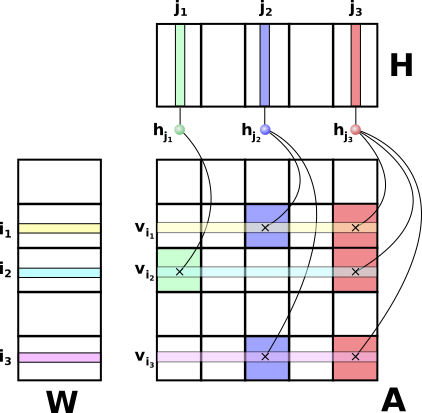
\includegraphics[width=0.8\linewidth]{figures/matrix-partition.png}
\end{figure}

\subsection{Partitioning}
\Cref{alg:distnmf} requires a partitioning of the nonzeros of $\Am$ as well as the rows and the columns of $\Wm$ and $\Hm$, and these three partitions completely determine its computational and communication costs.
Here, we compare different partitioning strategies, and argue how they relate to these two performance metrics.

Our algorithm is fine-grained; meaning that it can work any fine-grain, 1D, or 2D/checkerboard partition of the sparse matrix $\Am$.
Here, however, we exclusively focus on $P_r \times P_c$~(where $P = P_r P_c$) checkerboard partitionings, and always set $P_c$ to the number of cores available per compute node in the cluster.
This helps us reduce the communication cost in two ways.
The first one corresponds to that we do not employ shared-memory parallelism in our implementation, hence assign one MPI rank per core.
In this scenario, by assigning each group of $P_c$ processes owning the same row block of $\Am$ to the same node, and similarly assigning the corresponding row blocks of $\Wm$ and $\Wmt$ to these processes, we effectively eliminate the communication in the row dimension of the process grid~(which pertains to communicating matrices $\Wm$ and $\Wmt$) as these row exchanges stay within a node.
This enables us to focus solely on reducing the communication due to columns of $\Hm$ and $\Hmt$.
Second, this topology bounds the maximum number of messages sent per process by $P_r-1$ and $P_c-1$, thereby significantly reduce the communication latency by a factor of $P_c$ in compare with a fine-grain or a 1D partition, which incurs up to $P-1$ messages per process.

\subsubsection{Partitioning sparse input matrix $\Am$} \label{sec:cp1d}
\paragraph{Hypergraph partitioning~(\cpp)} We aim to partition the matrix $\Am$ into $P_r$ row slices first, and $P_c$ column slices next, to obtain an $P_r \times P_c$ checkerboard partition.
To this end, we adopt hypergraph partitioning techniques used in parallel sparse matrix literature to our case~\cite{caay:99}.
A hypergraph consists of vertices with associated weights and hyperedges that connect two or more vertices.
In the literature, a hypergraph is typically formed by adding a vertex for each computational task with the associated execution cost, adding a hyperedge for each data element, and connecting the vertex to a hyperedge whenever the associated task and the data are dependent.
Then, the vertices of the hypergraph is partitioned using a hypergraph partitioner to distribute vertex loads to parts equitably while reducing a metric called \emph{cutsize}, which amounts to minimizing the total number of different parts each hyperedge connects.
This corresponds in the actual computation to minimizing the data dependencies between tasks, hence the communication volume.
Here, we form a \emph{column-net} hypergraph model; for each row $i$ and column $j$ of  $\Am$, we add a vertex $v_i$ and a hyperedge $h_j$ to the hypergraph, and for each nonzero $(i, j) \in \Am$, which implies a dependency to $\Hm(:, j)$ in computing $\Wmt(i, :)$ at \cref{line:ah}, we connect $v_i$ to $h_j$.
We assign the value $(nnz(\Am) / m + nnz(\Am(i, :))$ to each vertex $v_i$.
This weighting is preferred to find a tradeoff between balancing the number of vertices, which corresponds to the cost of dense matrix operations, and balancing the number of nonzeros per part, which corresponds to the cost of sparse matrix-dense matrix multiplication.
We establish these two load balance goals by assigning a fixed cost to each vertex in the first summand, and increasing the cost of the vertices corresponding to denser rows in the second summand.
We then partition this hypergraph into $R$ parts by balancing the vertex weights, and minimizing the cutsize of the hypergraph.
In \cref{fig:partition} we also show this hypergraph construction for a $3 \times 3$ subset of the $A$ where rows corresponding to each vertex are highlighted and connected to related hyperedges.
In this partitioning, minimizing the cutsize of this hypergraph exactly corresponds to minimizing the total communication volume due to columns of $\Hm$ and $\Hmt$ as is clear in \cref{fig:partition}, whereas balancing the vertex weights corresponds to balancing the cost of sparse matrix-dense matrix multiplications as well as dense matrix operations in computing Gram matrices and $\textsc{Nnls}$ in each process row.

Once the matrix is partitioned into $R$ row slices, one can similarly partition columns of $\Am$ into $C$ parts using a multi-constraint formulation~\cite{aycu:08} using a \emph{row-net} hypergraph.
Yet in our case, we skip this common approach for two reasons.
First, existing multi-constraint partitioning tools are known to be not as efficient nor effective as single-constraint partitioners in practice.
Second, the main goal of hypergraph partitioning of columns is to minimize the communication volume due to rows, whereas in our case communication of rows of $\Wm$ and $\Wmt$ stays within a node with a proper mapping of processes, and this communication cost would be negligible.
Therefore, we instead partition columns randomly, which is expected to provide balance the number of nonzeros of $\Am$, number of columns of $\Hm$ and $\Hmt$, the amount of column communication volume due to columns of $\Hm$ and $\Hmt$.

\paragraph{Randomized checkerboard partitioning(\crp)}
This scheme corresponds to partitioning both the rows and the columns of $\Am$ into $R$ segments randomly.
It is expected to provide good load balance both in sparse and dense matrix operations, but it overlooks the communication cost.

\paragraph{Uniform checkerboard partitioning(\unp)}
This partitioning variant forms an $R \times C$ partition of $\Am$ by putting a contiguous set of $m / R$ and $n / C$ rows and columns in each slice.
$\Wm$ and $\Hm$ are partitioned conformally with this topology; each process is assigned a contiguous set of  $m / P$ and $n / P$ rows and columns, respectively, belonging to the corresponding row and column blocks of $\Hm$.
This is the only partitioning scheme employed by $\mpifaun$ \cite{KBP16, KBP16MPIFAUN}, hence we only use it for this implementation.
We also use a randomized variant (\urp) of this scheme in which the rows and columns of $\Am$ are permuted randomly befor executing $\mpifaun$ to better balance its nonzeros.

\subsubsection{Partitioning factors $\Wm$ and $\Hm$}
Once $\Am$ is partitioned with an $R \times C$ checkerboard topology, one has to partition rows and columns of factor matrices conformally with this topology to form the sets $\Ip$ and $\Jp$ in \cref{alg:distnmf}.
In doing so, we are interested in assigning rows and columns to processes in the corresponding process row or column equitably.
For this purpose, we specify imbalance parameters $\alpha_r$ and $\alpha_c$ that correspond to maximum imbalance we allow in this partitioning; i.e., $|\Ip| \le \alpha_r m / P$ and $|\Jp| \le \alpha_c n / P$ for each process $p$.
We normally set these imbalance parameters to $1.1$.
However, when $m >> n$, we increase $\alpha_c$ proportionally in order to give more flexibility in column partitioning which results in smaller communication volume.

Next, for each row and column of $\Wm$ and $\Hm$ we create a list of processes that has a dependency to that row or column, which corresponds to processes owning the matrix blocks of same color in \cref{fig:partition}.
Finally, we randomly assign each row and column to one of the processes satisfying the imbalance constraint in this list.
If all processes in the list are overloaded, we randomly assign it to a process that is not overloaded in the same process row or column.
Note that the latter assignment increases the communication volume due to that row or column by 1; hence, in general larger imbalance parameters yield smaller communication volume by reducing this type of assignment.

%%\newcommand{\smaller}{\scriptsize}
%\begin{table*}[t!]
%\begin{center}
%\begin{tabular}{|c|c|c|c|c|}
%\hline
%\textbf{Algorithm} & \textbf{Flops} & \textbf{Words} & \textbf{Messages} & \textbf{Memory}  \\ \hline
%\smaller \mpifaun ($m/p < n$) & \smaller $O(2*nnz_p*k)+\frac{(m+n)k^2}{p}+F\lt(\frac mp,\frac np,k\rt)$ & \smaller $O\lt( \sqrt{\frac{mnk^2}{p}}\rt)$ & \smaller $O(\log p)^*$ & \smaller $O\lt(\frac{mn}{p}+\sqrt{\frac{mnk^2}{p}}\rt)$ \\ \hline
%\end{tabular}
%\normalsize
%\end{center}
%\caption{Leading order algorithmic costs for \NaiveAlg{} and \ParNMF{} (per iteration).  
%The function $F(\cdot)$ denotes the number of flops required for the particular NMF algorithm's Local Update Computation, aside from the matrix multiplications common across AU-NMF algorithms. \\
%$^*$The stated latency cost assumes no communication is required in \LUC; \HALS\ requires $k\log p$ messages for normalization steps.}
%\label{tab:costs}
%\end{table*}%
